\chapter{Matematik}
%%
%%
\section*{Polære Koordinater, Cosinus og Sinus}
%%
%%
\begin{opgave}{Idiotformlen}{1}
Man kalder oftest udtrykket $\cos^2(\theta)+\sin^2(\theta)=1$ for idiotformlen, da man ofte glemmer den. Vis hvorfor dette udtryk er gældende ud fra definitionen af sinus og cosinus samt Pythagoras sætning.
\end{opgave}
%%
%%
\begin{opgave}{Tangens}{1}
Vi betragter en retvinklet trekant med to kateter, den hosliggende katete $a$ og den modstående katete $b$, samt en hypotenuse $c$.
\opg Vis hvorfor $\tan(\theta)=b/a$ ud fra definitionen af sinus og cosinus.
\opg For $\tan(\theta)=1$, find $\theta$.
\end{opgave}
%%
%%
\begin{opgave}{Retvinklede trekanter}{1}
En retvinklet trekant har to kateter $a,b$ og en hypotenuse $c$. Vi antager at længderne af $a$ og $c$ er hhv. $5$ og $13$.
\opg Bestem vinklen mellem $a$ og $c$ vha. cosinus.
\opg Bestem længden af $b$ vha. tangens.
\opg Bestem vinklen mellem $b$ og $c$ vha. sinus.
\end{opgave}
%%
%%
\begin{opgave}{Koordinatskift}{1}
Omskriv følgende punkter skrevet i kartesiske koordinater til polære koordinater. Dvs. find $r$ og $\theta$ vha. de givne $x$ og $y$. Lav også en lille skitse af punkterne i et $xy$-koordinatsystem, hvor $r$ og $\theta$ indtegnes.
\opg $x=2$ og $y=2$.
\opg $x=1$ og $y=-2$.\\
I 2) vælger man selv, om man vil regne $\theta$ som positiv (mod uret) eller negativ (med uret) ift. $x$-aksen.
\end{opgave}
%%
%%
\begin{opgave}{Koordinatskift 2}{1}
Omskriv følgende punkter skrevet i polære koordinater til kartetiske koordinater, og lav en lille skitse af punkterne i et $xy$-koordinatsystem.
\opg $r=5$ og $\theta=\frac{\pi}{4}$.
\opg $r=5$ og $\theta=\frac{7\pi}{4}$.
\opg $r=13$ og $\theta=\frac{11\pi}{6}$.
\end{opgave}
%%
%%
\newpage
\section*{Differentialregning}
%%
%%
\begin{opgave}{Hastighed og postion}{1}
	\begin{figure}[h!]
		\centering
		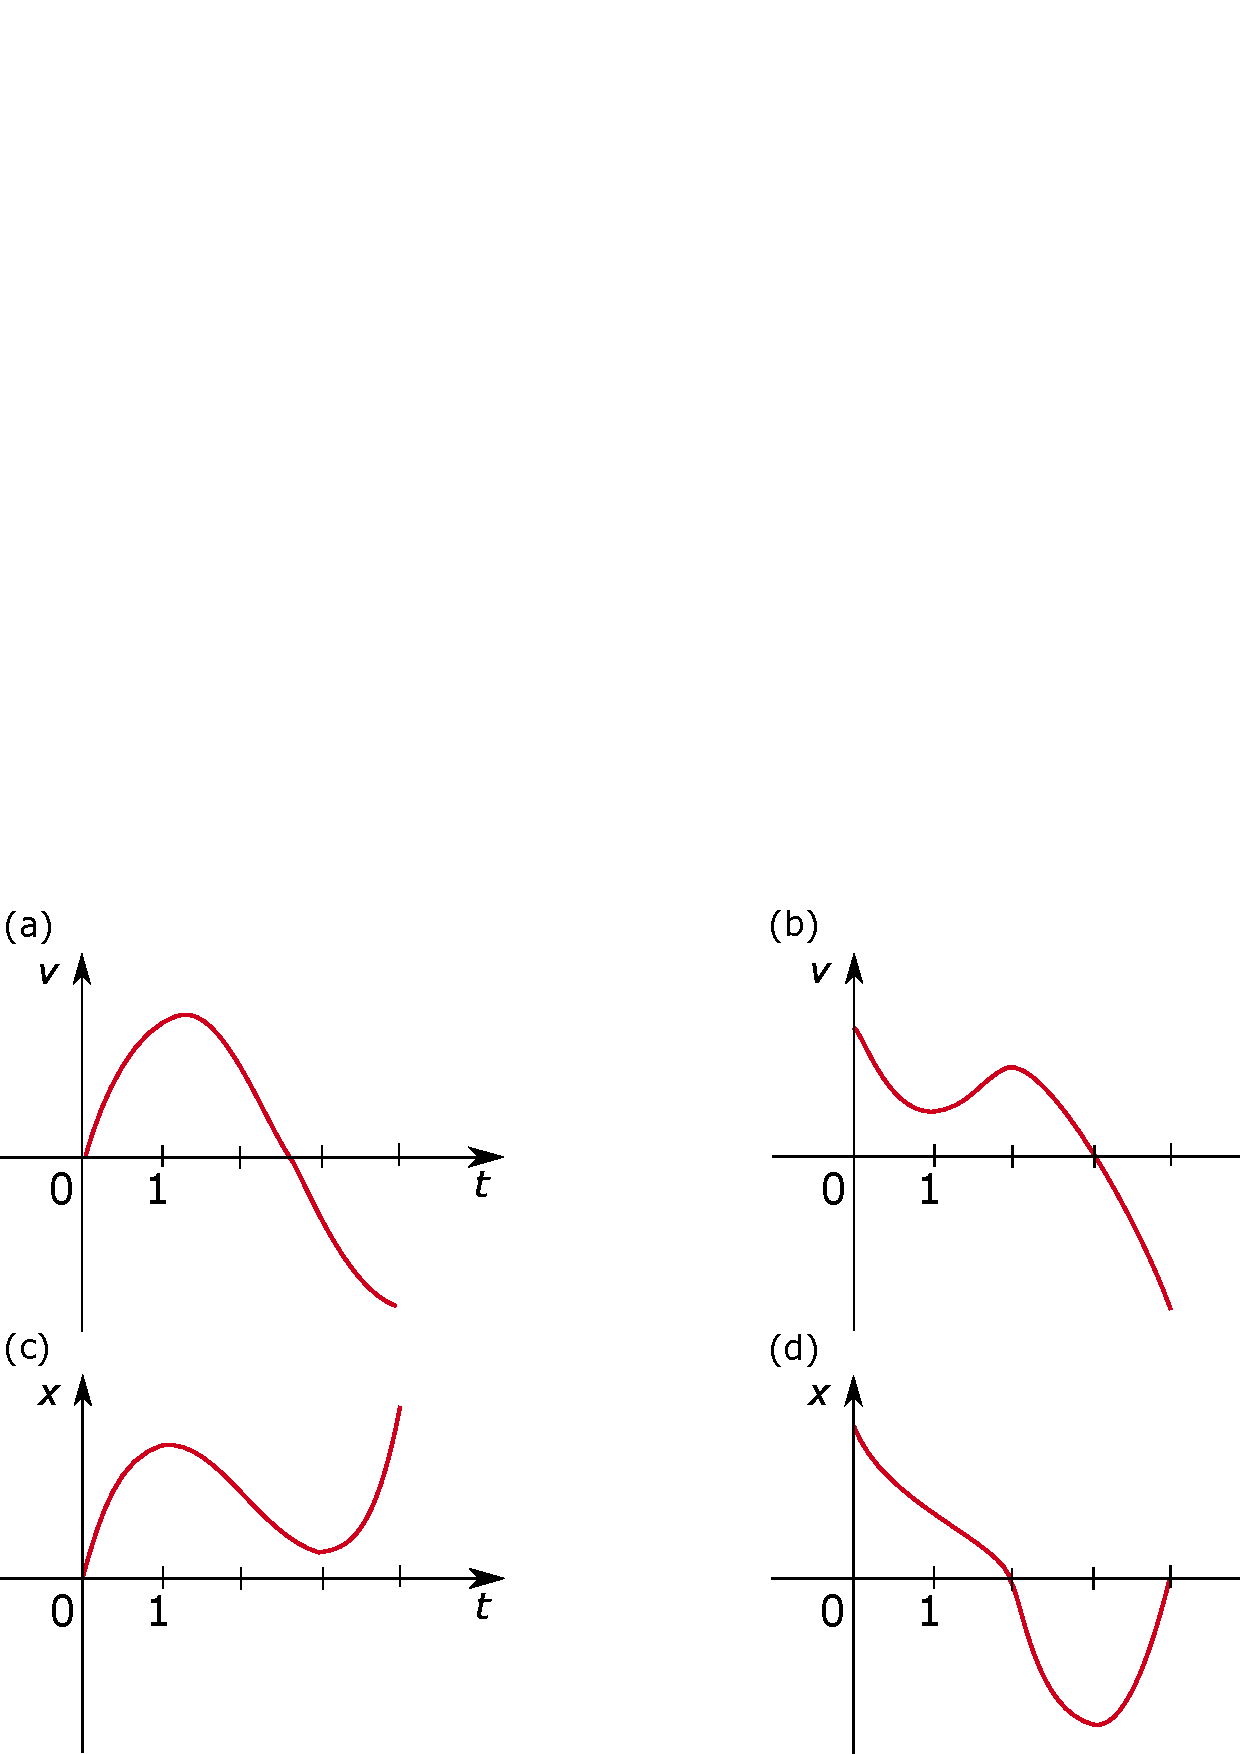
\includegraphics[width=0.47\textwidth]{matematik/vx_grafer.png}
		\caption{Hastighed og position som funktion af tiden.}
		\label{fig:vx_grafer}
	\end{figure}
	\opg Figur \ref{fig:vx_grafer} (a) og (b) viser hastigheden af to objekter som funktion af tiden i sekunder. Hvornår sætter de to objekter hastigheden op, og hvornår sætter de hastigheden ned? Forklar dit svar.
	\opg Figur \ref{fig:vx_grafer} (c) og (d) viser positionen af to objekter $x$ som funktion af tiden i sekunder. Hvornår sætter de to objekter hastigheden op, og hvornår sætter de hastigheden ned? Forklar dit svar.\\
\end{opgave}
%%
%%
\begin{opgave}{Afledede og dobbeltafledede}{1}
Find den afledede og dobbeltafledede med hensyn til $x$ for følgende funktioner:
\opg $f(x) = x^3.$
\opg $f(x) = x^2 + 4x.$
\opg $f(x) = \frac{1}{x} + \frac{1}{x^2}.$
\opg $f(x) = \cos(x).$
\opg $f(x) = \ln(x).$
\opg $f(x) = x \sin(x).$
\opg $f(x) = \frac{1}{x} \ln(x).$ \\
\end{opgave}
%%
%%
\begin{opgave}{Sammensatte funktioner}{1}
Skriv følgende udtryk som en sammensat funktion $f(g(x)$ (altså skal du identificere den indre funktion $g(x)$ og den ydre funktion $f(g)$). Beregn derefter $\dif{x}{f}$. 
\opg $f(x) = \sin (4x).$
\opg $f(x) = \sqrt{2x}.$
\opg $f(x) = \sqrt{4x+5}.$
\opg $f(x) = \sin(e^x).$
\opg $f(x) =  \ln \left( \cos x \right).$ \\
\end{opgave}
%%
%%
\begin{opgave}{Funktioner af flere variable - partiel differentiering}{2}
I denne opgave skal vi kigge på partiel differentiering og kigger som et eksempel på funktioner af tre variable $f(x,y,z)$. For hver af de følgende funktioner skal I beregne den partielt afledede ift. både $x$, $y$ og $z$.
\opg $f(x,y,z) = x +y^2 + z^3.$
\opg $f(x,y,z) = x y^2 +  ye^{-z}.$
\opg $f(x,y,z) = ze^{xyz}.$
\opg $f(x,y,z) = \frac{x-y+5z}{x+y+z}.$ \\
\end{opgave}
%%
%%
\begin{opgave}{Funktioner af flere variable - total differentiering}{3}
	I denne opgave skal vi kigge på total differentiering og kigger som et eksempel på funktioner af fire variable $f(x,y,z,t)$. Vi antager at de tre første variable $x,y,z$ afhænger af den fjerde $t$, altså $x(t)$, $y(t)$ og $z(t)$. I skal nu beregne den totalt differentierede $\dif{t}{f}$ for følgende funktioner.\\
	Hint: Brug formel \eqref{k-total_dif} i matematikafsnittet og resultaterne fra forrige opgave i 2) og 3).\\
	\opg $f(x,y,z,t) = xyz.$ 
	\opg $f(x,y,z,t) = x +y^2 + z^3.$
	\opg $f(x,y,z,t) = x y^2 +  ye^{-z}.$
	\opg Diskuter hvad der sker i resultaterne for 1)-3), hvis variablene $x,y,z$ ikke afhænger af $t$. \\
\end{opgave}
%%
%%
\section*{Integralregning}
%%
%%
\begin{opgave}{Integraler og arealer under funktioner}{1}
I matematikafsnittet i kompendiet nævnes det, at når man regner et bestemt integrale
\begin{equation*}
\integral{f(x)}{x}{a}{b} \, ,
\end{equation*}
så er svaret det samme som arealet under grafen for $f(x)$ i intervallet $[a,b]$ på $x$-aksen. Brug dette faktum til at diskutere den fysiske forståelse af følgende udsagn.
\opg Hvis man integrerer en hastighed $v(t)$ ift. tiden $t$, så får man en position $x(t)$.
\opg Hvis man integrerer en acceleration $a(t)$ ift. tiden $t$, så får man en hastighed $v(t)$. \\
\end{opgave}
%%
%%
\begin{opgave}{Ubestemte integraler}{1}
	Udregn det ubestemte integrale af følgende funktioner:
	\opg $f(x) = x^3$.
	\opg $f(x) = x^2 + 4x$.
	\opg $f(x) = \frac{1}{x} + \frac{1}{x^2}$.
	\opg $f(x) = \cos (x)$.
	\opg $f(x) = \ln (x)$.
\end{opgave}
%%
%%
\begin{opgave}{Integration ved substitution}{2}
	Udregn de følgende integraler vha. integration ved substitution:
	\opg $\integral{e^{-4x}}{x}{}{}$.
	\opg $\integral{\sqrt{3x-2}}{x}{}{}$.
	\opg $\integral{xe^{-3x^2}}{x}{}{}$.
	\opg $\integral{\frac{x-1}{\sqrt{x+1}}}{x}{}{}$.
\end{opgave}
%%
%%
\begin{opgave}{Partiel integration}{3}
	Udregn de følgende integrale vha. partiel integration:
	\opg $\integral{4x\cos(2-3x)}{x}{}{}$.
	\opg $\integral{(2+5x)e^{\frac{1}{3}x}}{x}{}{}$.
	\opg $\integral{(3x+x^2)\sin (2x)}{x}{}{}$.
\end{opgave}
%%
%%
\section*{Differentialligninger}
%%
%%
\begin{opgave}{Specialtilfælde af 1. og 2. ordens differentialligninger}{1}
I denne opgave skal I vise, at nogle forskellige funktioner er løsninger til de givne differentialligninger.
\opg Vis at funktionen $f(t) = -7e^{3t}$ løser differentialligningen 
\begin{align*}
\dif{t}{f} = 3 f(t) \, .
\end{align*}
\opg Vis at funktionen $g(t) = \frac{2}{3}e^t + e^{-2t}$ løser differentialligningen
\begin{align*}
\dif{t}{g} +2g(t) = 2e^t \, .
\end{align*}
\opg Vis at funktionen $h(t) = 5 \sin (3t) - 10 \cos(3t)$ løser differentialligningen
\begin{align*}
\dif[2]{t}{h} = -9h(t) \, .
\end{align*}
\opg Tjek om funktionen $k(t) = 13 \cos (8t + 45)$ løser differentialligningen
\begin{align*}
\dif[2]{t}{k} = -64k(t) \, .
\end{align*}
\end{opgave}
%%
%%
\begin{opgave}{Generelle 1. ordens differentialligninger.}{2}
I denne opgave skal I også vise, at nogle forskellige funktioner er løsninger til de givne differentialligninger. Denne gang er funktionerne og differentialligningerne dog skrevet op på en mere generel form, dvs. at de kan indeholde arbitrære konstanter.
\opg Vis at alle funktioner på formen
\begin{align*}
	h(x) = \frac{1}{x + A} 
\end{align*}
løser differentialligningen
\begin{align*}
	\dif{x}{h} = - h(x)^2 \; .
\end{align*}
\opg Vis at alle funktioner på formen
\begin{align*}
	k(x) = \left( c - x^2 \right)^{-1/2}
\end{align*}
løser differentialligningen
\begin{align*}
	\dif{x}{k} = x k(x)^3 \; .
\end{align*}
\opg Vis at alle funktioner på formen
\begin{align*}
	g(x) = \frac{\ln (x) + C}{x}
\end{align*}
løser differentialligningen
\begin{align*}
	x^2 \dif{x}{g} + xg(x) = 1 \; .
\end{align*} 
\opg Vis at alle funktioner på formen
\begin{align*}
	f(x) = \frac{1 + ce^x}{1-ce^x}
\end{align*}
løser differentialligningen
\begin{align*}
	\dif{x}{f} = \frac{1}{2} \left( f(x)^2 - 1 \right) \; .
\end{align*} 
\end{opgave}
%%
%%
\begin{opgave}{Hvornår er det en løsning?}{3}
	I denne opgave skal I finde ud af, hvornår nogle forskellige funktioner er løsninger til de givne differentialligninger. Sagt med andre ord skal I finde de specifikke værdier for nogle af de konstanter, der indgår i funktionerne, som gør at funktionerne løser differentialligningerne.
	\opg For hvilke værdier af $k$ løser funktionen
	\begin{align*}
	f(y) = \cos (ky)
	\end{align*}
	differentialligningen
	\begin{align*}
	4 \dif[2]{y}{f} = - 25f(y) \, .
	\end{align*}
	\opg Tjek for de værdier af $k$ I fandt i 1), at funktionen $g(y) = A \sin (ky) + B \cos (ky)$ også løser differentialligningen
	\begin{align*}
	4 \dif[2]{y}{g} = -25 g(y) \, .
	\end{align*}
	\opg For hvilke værdier af $r$ løser funktionen
	\begin{align*}
	h(y) = e^{ry}
	\end{align*}
	differentialligningen
	\begin{align*}
	2 \dif[2]{y}{h} + \dif{y}{h} - h(y) = 0 \, .
	\end{align*}
	\opg Lad $r_1$ og $r_2$ være de konstanter du fandt i 3). Tjek at funktionen $k (y) = ae^{r_1y} + be^{r_2y} $ også løser differentialligningen
	\begin{align*}
	2 \dif[2]{y}{k} + \dif{y}{k} - k(y) = 0 \, .
	\end{align*}
\end{opgave}
%%
%%
\section*{Taylorapproksimationer}
%%
%%
\begin{opgave}{Approksimation af funktion}{1}
	I denne opgave skal I prøve at kigge lidt nærmere på Taylorapproksimationer, og hvad det egentligt er for en størrelse. Dette skal gøres på baggrund af formel \eqref{k-Taylor_pol} fra matematikafsnittet i kompendiet.
	\opg Diskuter betydningen af de enkelte led i summen. Hvordan ser de
	ud som funktioner af $x$, og hvorfor bliver approksimationen bedre
	af at tage flere led med?
\end{opgave}	
%%
%%
\begin{opgave}{Taylorpolynomier for simple funktioner}{2}
I denne opgave skal I bestemme Taylorpolynomierne $T_0(x)$, $T_1(x)$ og $T_2(x)$ for følgende funktioner vha. formel \eqref{k-Taylor_pol} i kompendiet.
\opg $f(x) = \cos(x)$.
\opg $f(x) = \sin(x)$.
\opg $f(x) = e^x$.
\opg Indsæt nu $a=0$ i jeres resultater for $T_2(x)$ i 1)-3), og tjek om svaret stemmer med Taylorpolynomierne i tabel \ref{k-Taylorseries_table} i matematikafsnittet i kompendiet. 
\end{opgave}
%%
%%
\begin{opgave}{Jordens form}{3}
Betragt nu funktionen
\begin{align*}
f(x) = \sqrt{R^2 - x^2} \, ,
\end{align*}
hvor $ x \in [-R,R]$ og $R$ er en positiv konstant.
\opg Bestem Taylorpolynomierne for $f(x)$ til 0., 1. og 2. orden omkring $x=0$.
\opg Hvilke typer af funktioner giver hver approksimationsorden?
\opg Funktionen $f(x)$ beskriver den øvre del af en cirkel med centrum i origo, $(0,0)$, i et $xy$-koordinatsystem, hvor $y = f(x)$. Den nedre del fås ved at sætte et negativt fortegn på, dvs. $g(x) = -f(x)$. Skitser $f(x)$ og $g(x)$, samt approksimationerne af de to funktioner til 0., 1., og 2. orden for $x \in [-R,R]$.\\
Hint: Approksimationerne af $g(x)$ er de samme som for $f(x)$ men med det modsatte fortegn. 
\opg Antag at resultaterne fra 3) generaliserer til tre dimensioner, dvs. en funktion af to variable $f(x,y)$\footnote{Taylorrækken for en funktion af $n$ variable kan i ord beskrives som en sum af $n$ Taylorrækker, hvor der bruges partielt afledede. Det er super grimt at skrive op, men fungerer på samme måde som for én variabel.}, der beskriver overfladen af den øvre halvdel af en sfære. Hvilke geometriske objekter får man da for hver af de 3 approksimationsordner, hvis der udvikles omkring $(x,y)=(0,0)$?
\opg Brug dette til, under antagelse af at Jorden kan beskrives som en perfekt sfære, at konkludere, hvilke andre geometriske former Jorden kan anses for at have, hvis man nu kun forstod verden til de lavere approksimationsordner.
\end{opgave}
%%
%%
\section*{Komplekse tal}
%%
%%
\begin{opgave}{Den komplekse plan}{1}
Tegn følgende komplekse tal i den komplekse plan.
\opg $z = 5$.
\opg $z = -3i$.
\opg $z = 4 + 7i$.
\opg $z = -3 - 2i$.
\end{opgave}
%%
%%
\begin{opgave}{Regning med komplekse tal}{1}
I denne opgave kigger vi på de komplekse tal:
\begin{align*}
z_1 &= 3 + 2i \, , \\
z_2 &= -6+i \, , \\ 
z_3 &= 1 - 5i \, , \\
z_4 &= -4 + 3i \, .
\end{align*}
\opg Beregn $z_1+z_2$ og $z_3+z_4$.
\opg Beregn $z_1-z_2$ og $z_3-z_4$.
\opg Beregn $z_1z_2$ og $z_3z_4$.
\opg Beregn $z_1/z_2$ og $z_3/z_4$.
\opg Beregn $\abs{z_1}$ og $\abs{z_2}$ samt $\abs{z_3 z_4}^2$. 
\end{opgave}
%%
%%
\begin{opgave}{Regneregler for modulus og normkvadratet}{2}
I denne opgave skal vi kigge på de regneregler for modulus samt normkvadratet for komplekse tal, der er  præsenteret i matematikafsnittet.
\opg Eftervis formlerne for modulus \eqref{k-modulus_regneregler1}, \eqref{k-modulus_regneregler2} og \eqref{k-modulus_regneregler3}.
\opg Eftervis formlen for normkvadratet \eqref{k-normkvadrat}.\\ \\  
\end{opgave}
%%
%%
\begin{opgave}{Eulers formel og komplekse tal på polær form}{3}
Her skal vi arbejde med Eulers formel og prøve at få lidt intuition for, hvordan funktionen $e^{ix}$ opfører sig. I 5) skal I videre kigge på det, der kaldes for den polære form for komplekse tal.
\opg Tegn det komplekse tal $e^{ix}$ vha. Eulers formel \eqref{k-Eulers_formel} fra matematikafsnittet for $x=0, \, \pi/2, \, \pi,3\pi/2$ (hvis ens lommeregner regner i grader for $\cos(x)$ og $\sin(x)$ skal man bruge $x=0, \, 90, \, 180, \, 270$ i stedet). Hvilken vej bevæger $e^{ix}$ sig rundt i den komplekse plan, når $x$ vokser?
\opg Ændres modulus af $e^{ix}$, hvis man ændre på $x$? Hint: Regn modulus af $e^{ix}$ vha. Eulers formel.
\opg Hvilken vej tror du, at $e^{-ix}$ bevæger sig rundt i den komplekse plan, når $x$ vokser?
\opg Ændres modulus af $e^{-ix}$, hvis man ændre $x$?
\opg Vis at ethvert komplekst tal $z = a+bi$ kan skrives på følgende form
\begin{align}
z = \abs{z}e^{i\theta} \, ,
\end{align} 
hvor $\theta = \arctan(b/a)$. Her er $\theta$ vinklen mellem den reelle akse og $z$ i det komplekse plan, og kaldes for $z$'s argument. I skal altså starte med $z=a+bi$ og omskrive, indtil i får noget på formen $|z|e^{i\theta}$. Denne måde at skrive et komplekst tal kaldes for den polære form.\\
Hint: Tegn $z$ i det komplekse plan og udtryk $a,b$ ved $\abs{z},\theta$ før I begynder at skrive om.
\end{opgave}
%%
%%
\begin{opgave}{Komplekse ligninger}{2}
Løs de følgende komplekse ligninger for $z$.
\opg $\frac{z-2}{z+1} = 3i$.
\opg $z+3z^* = 5-6i$.
\end{opgave}
%%
%%
\section*{Vektorer}
%%
%%
\begin{opgave}{Længden af en vektor}{1} 
Beregn længden af de to vektorer
\begin{align*}
\v{v}_1 = \begin{bmatrix} 1 \\ 2 \\ 3 \end{bmatrix} \, , \quad \v{v}_2 = \begin{bmatrix} -4 \\ 5 \\ 0  \end{bmatrix} \, .
\end{align*}
\end{opgave}
%%
%%
\begin{opgave}{Addition, subtraktion og skalarmultiplikation med vektorer}{1}
Her vil vi kigge på, hvordan man lægger/trækker vektorer til/fra hinanden, og hvordan man ganger en vektor med en skalar (et tal). I denne opgave genbruger vi de to vektorer fra forrige opgave 
\opg Bestem $\v{v}_1 + \v{v}_2$.
\opg Bestem $\v{v}_1 - \v{v}_2$.
\opg Bestem $5 \cdot \v{v}_1$ og $5 \cdot \v{v}_2$.
\opg Bestem $5 \cdot \left( \v{v}_1 \pm \v{v}_2 \right)$ og sammenlign med $5 \cdot \v{v}_1 \pm 5 \cdot \v{v}_2$. Hvad betyder dette resultat?
\end{opgave}
%%
%%
\begin{opgave}{Skalarproduktet}{2}
Nu skal vi kigge på, hvordan man ganger med vektorer, og starter med skalarproduktet. Igen bruger vi vektorerne fra forrige opgave.
\opg Bestem $\v{v}_1 \cdot \v{v}_2$ og sammenlign med $\v{v}_2 \cdot \v{v}_1$. Har rækkefølgen af vektorerne betydning?
\opg Tjek formlen $\abs{\v{v}} = \sqrt{\v{v} \cdot \v{v}}$ for $\v{v}_1$ og $\v{v}_2$.
\opg Brug formel \eqref{k-skalarproduct-angle} til at bestemme vinklen $\theta$ mellem $\v{v}_1$ og $\v{v}_2$.
\opg Hvad betyder det for vinklen $\theta$ mellem to vektorer $\v{v}_1$ og $\v{v}_2$, hvis skalarproduktet $\v{v}_1 \cdot \v{v}_2 = 0$ og $\abs{\v{v}_1},\abs{\v{v}_2} \neq 0$?\\  
\end{opgave}
%%
%%
\begin{opgave}{Krydsproduktet}{2}
Vi kigger nu på krydsproduktet og genbruger atter vektorerne fra tidligere.
\opg Bestem $\v{v}_1 \times \v{v}_2$ og sammenlign med $\v{v}_2 \times \v{v}_1$. Har rækkefølgen af vektorerne i et krydsprodukt nogen betydning? 
\opg Bestem $\abs{\v{v}_1 \times \v{v}_2}$.
\opg Brug formel \eqref{k-crossproduct-angle} til at bestemme vinklen mellem $\v{v}_1$ og $\v{v}_2$. Tjek at dit svar stemmer med resultatet du fandt i forrige opgave.
\opg Hvad betyder det for vinklen $\theta$ mellem to vektorer $\v{v}_1$ og $\v{v}_2$, hvis krydsproduktet $\v{v}_1 \times \v{v}_2 = 0$ og $\abs{\v{v}_1},\abs{\v{v}_2} \neq 0$? 
\end{opgave}
%%
%%
\begin{opgave}{Regning med enhedsvektorer}{2}
I denne opgave vil vi kigge lidt på, hvordan man kan regne med vektorer $\v{v}_1$ og  $\v{v_2}$, når disse skrives vha. enhedsvektorer. Vi vælger her at skrive vores vektorer på en generel form
\begin{align*}
\v{v}_1 = \begin{bmatrix} v_{x_1} \\ v_{y_1} \\ v_{z_1} \end{bmatrix} \, , \quad \v{v}_2 = \begin{bmatrix} v_{x_2} \\ v_{y_2} \\ v_{z_2} \end{bmatrix}  \, .
\end{align*}
\opg Opskriv $\v{v}_1$ og $\v{v}_2$ vha. enhedsvektorerne $\xhat,\yhat,\zhat$.
\opg Tjek at
\begin{align*}
\v{v}_1 \pm \v{v}_2 = (v_{x_1} \pm v_{x_2}) \xhat + (v_{y_1} \pm v_{y_2}) \yhat + (v_{z_1} \pm v_{z_2}) \zhat \, .
\end{align*}
\opg Beregn de forskellige skalarprodukter mellem enhedsvektorerne $\xhat,\yhat,\zhat$. Altså $\xhat \cdot \xhat$, $\xhat \cdot \yhat$ osv.
\opg Brug resultaterne fra 3) til at beregne skalarproduktet vha. enhedsvektorer. Stemmer dit resultat med den normale formel for skalarproduktet?
\opg Beregn de forskellige krydsprodukter mellem enhedsvektorerne $\xhat,\yhat,\zhat$. Altså $\xhat \times \xhat$, $\xhat \times \yhat$ osv.
\opg Brug resultaterne fra 5) til at beregne krydsproduktet vha. enhedsvektorer. Stemmer dit resultat?
\end{opgave}
%%
%%